\documentclass[tikz,border=10pt]{standalone}
\usetikzlibrary{calc, intersections}

\begin{document}
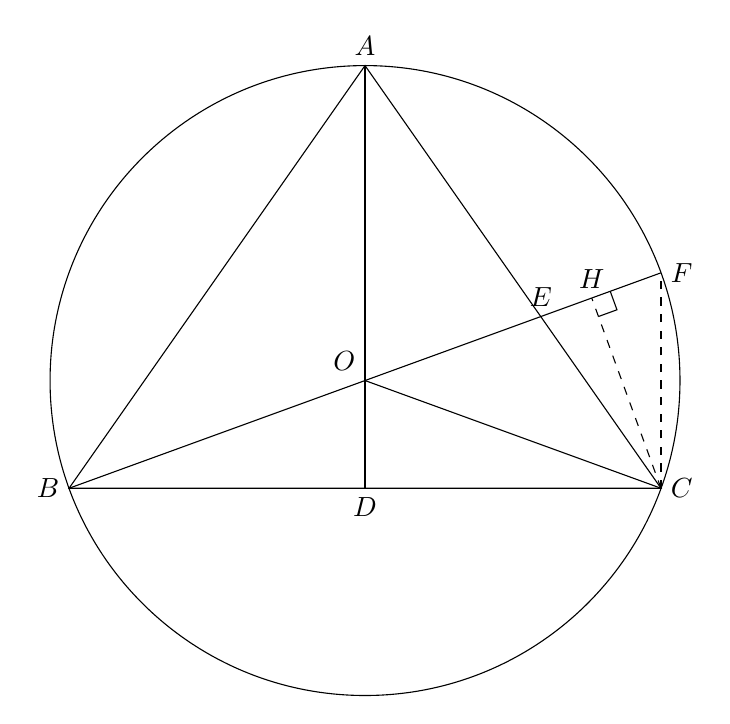
\begin{tikzpicture}
    % Define coordinates
    \coordinate (O) at (0,0);
    \def\R{4}
    \def\alpha{20} % degrees

    % Points on circle
    \coordinate (A) at (90:\R);
    \coordinate (B) at (180+\alpha:\R);
    \coordinate (C) at (360-\alpha:\R);
    \coordinate (F) at (\alpha:\R);

    % Point D (intersection of BC and vertical axis)
    \coordinate (D) at (0, {- \R * sin(\alpha)});

    % Intersection E (AC and BF)
    \path[name path=AC] (A) -- (C);
    \path[name path=BF] (B) -- (F);
    \path[name intersections={of=AC and BF, by=E}];

    % Point H (Projection of C onto BF)
    \coordinate (H) at ($(B)!(C)!(F)$);

    % Draw Circle
    \draw (O) circle (\R);

    % Draw Triangle ABC
    \draw (A) -- (B) -- (C) -- cycle;

    % Draw Line AD (vertical)
    \draw (A) -- (D);

    % Draw Line BF (diameter)
    \draw (B) -- (F);

    % Draw Line OC
    \draw (O) -- (C);

    % Draw Dashed Lines
    \draw[dashed] (C) -- (H);
    \draw[dashed] (C) -- (F);

    % Draw Right Angle at H
    \def\ralen{0.25cm}
    \coordinate (P1) at ($(H)!\ralen!(F)$);
    \coordinate (P2) at ($(H)!\ralen!(C)$);
    \draw (P1) -- ($(P1)+(P2)-(H)$) -- (P2);

    % Labels
    \node[above] at (A) {$A$};
    \node[left] at (B) {$B$};
    \node[right] at (C) {$C$};
    \node[below] at (D) {$D$};
    \node[above left] at (O) {$O$};
    \node[above] at (E) {$E$};
    \node[above] at (H) {$H$};
    \node[right] at (F) {$F$};

\end{tikzpicture}
\end{document}
